\documentclass{standalone}

% graphics
\usepackage{tikz}
\usepackage{pgfplots}
\usepackage{siunitx}

\begin{document}

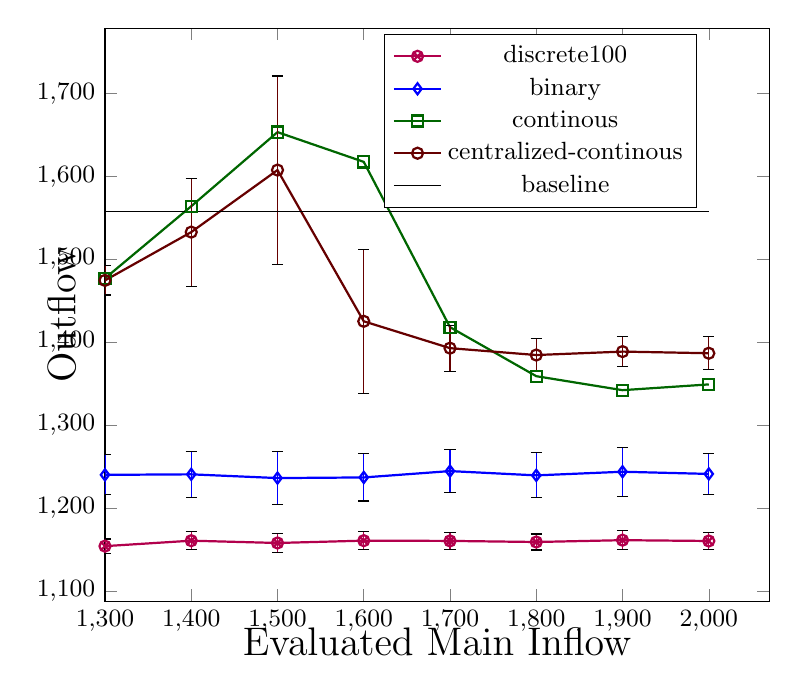
\begin{tikzpicture}[scale=1]
  \pgfplotsset{
      scale only axis,
      every x tick label/.append style={font=\small},
      every y tick label/.append style={font=\small},
	legend style={at={(0.42,0.99)},anchor=north west}
  }

\begin{axis}[
    legend style={font=\small},
	ylabel={\Large Outflow},
	x label style={at={(axis description cs:0.5,-0.03)},anchor=north},
	y label style={at={(axis description cs:-0.030,0.5)}, anchor=south},
	xlabel={\Large Evaluated Main Inflow},
	xmin=1300
]

%densely dashed, 
%discrete100
\addplot[mark=otimes, thick, mark options={solid, fill=red!60, mark size=2pt},
draw=red!70!blue, error bars/.cd, y dir=both, y explicit] table [x=a, y=b, y error=c] {
a	b   	c
1300 1154.20 8.67
1400 1160.78 10.56
1500 1158.01 11.85
1600 1160.82 10.72
1700 1160.50 10.47
1800 1159.20 9.62
1900 1161.40 11.20
2000 1160.42 9.73
};
\label{discrete100}

% dashdotdotted,
%binary 
\addplot[mark=diamond, thick, mark options={solid, fill=blue!40, mark size=2 pt}, draw=blue, error bars/.cd, y dir=both, y explicit] table [x=a, y=b, y error=c] {
a	b   	c
1300 1240.16 24.18
1400 1240.78 27.77
1500 1236.28 31.69
1600 1237.03 28.43
1700 1244.70 25.70
1800 1239.52 27.18
1900 1243.91 29.46
2000 1241.28 24.63
};
\label{binary}

% error bars/.cd, y dir=both, y explicit,
% continuos 
\addplot[mark=square, thick, mark options={solid, fill=green!60, mark size=2 pt}, draw=black!60!green] table [x=a, y=b] {
a	b   	c
1300 1477.08 14.37
1400 1564.02 9.06
1500 1653.37 58.17
1600 1617.52 169.13
1700 1418.22 96.92
1800 1359.11 39.57
1900 1342.26 28.89
2000 1349.21 30.17
};
\label{continous}  

%densely dashed, 
%centralized continous 
\addplot[mark=o, thick, mark options={solid, fill=black!60!red, mark size=2pt}, draw=black!60!red, error bars/.cd, y dir=both, y explicit] table [x=a, y=b, y error=c] {
a	b   	c
1300 1474.60 17.62
1400 1532.84 65.17
1500 1607.65 113.45
1600 1425.28 86.57
1700 1392.91 27.71
1800 1384.63 19.49
1900 1388.77 17.81
2000 1386.79 19.77
};
\label{centralized-continous}

%%densely dashed, 
%%main1400-1700_merge200
%\addplot[mark=triangle, thick, loosely dotted, mark options={solid, fill=red!60, mark size=2pt}, draw=black!20!red, error bars/.cd, y dir=both, y explicit] table [x=a, y=b, y error=c] {
%a	b   	c
%1300 1478.74 1.62
%1400 1573.70 2.39
%1500 1668.78 2.94
%1600 1762.27 9.53
%1700 1766.34 65.53
%1800 1722.06 33.99
%1900 1719.32 32.46
%2000 1714.28 27.98
%};
%\label{main1400-1700}

%%densely dashed, 
%\addplot[mark=otimes, thick, mark options={solid, fill=red!60, mark size=2pt},
%draw=blue!10!green, error bars/.cd, y dir=both, y explicit] table [x=a, y=b, y error=c] {
%a	b   	c
%
%};
%\label{AVP90}
%
%
%%densely dashed, 
%\addplot[mark=otimes, thick, mark options={solid, fill=blue!60, mark size=2pt},
%draw=blue!10!red, error bars/.cd, y dir=both, y explicit] table [x=a, y=b, y error=c] {
%a	b   	c
%
%};
%\label{linearPPO}
%

\addplot[mark=none, black, samples=200] coordinates {(1300,1558.12) (2000,1558.12)};
\label{baseline}


\addlegendimage{/pgfplots/refstyle=discrete100}
\addlegendentry{discrete100}

\addlegendimage{/pgfplots/refstyle=binary}
\addlegendentry{binary}

\addlegendimage{/pgfplots/refstyle=continous}
\addlegendentry{continous}

\addlegendimage{/pgfplots/refstyle=centralized-continous}
\addlegendentry{centralized-continous}

\addlegendimage{/pgfplots/refstyle=baseline}
\addlegendentry{baseline}


%\addlegendimage{/pgfplots/refstyle=AVP90}
%\addlegendentry{AVP90}

%\addlegendimage{/pgfplots/refstyle=linearPPO}
%\addlegendentry{linearPPOAVP10}

%\addlegendimage{/pgfplots/refstyle=Baseline}
%\addlegendentry{Human Baseline}

\end{axis}
\end{tikzpicture}

\end{document}

